%!TeX root = ../main.tex

{\raggedright\large\textbf{Local feature compression using autoencoders - SfM tests}}\smallskip \\ 
Design a compression strategy for local SURF descriptors using autoencoders. Training data can be generated using the images of dataset Portello and Castle. Testing must be done on dataset FountainP-11 and Tiso (available at \url{https://github.com/openMVG/SfM_quality_evaluation/tree/master/Benchmarking_Camera_Calibration_2008} and \url{http://www.dei.unipd.it/~sim1mil/materiale/3Drecon/}). Software must be implemented in MATLAB, Keras or Pytorch. \\ \textbf{Testing on 3D reconstruction using SfM:} The reconstructed descriptors (only for the test set) are used to perform a SfM reconstruction using COLMAP (using the two test dataset). \\
Programming languages: MATLAB/Python/C++.

\section{Introduction}

\subsection{What are the descriptors}
In computer vision, visual descriptors or image descriptors are descriptions of the visual features of the contents in images, videos, or algorithms or applications that produce such descriptions. They describe elementary characteristics such as the shape, the color, the texture or the motion, among others\footnote{\url{https://en.wikipedia.org/wiki/Visual_descriptor}, 01/02/21}. A feature detector (\emph{extractor}) is an algorithm taking an image as input and outputting a set of regions (``local features'' = ``Interest Points'' = ``Keypoints'' = ``Feature Points''). A descriptor is computed on an image region defined by a detector. The descriptor is a representation of the image function (colour, shape, ...) in the region (typically an array). Two key operations are related to feature extraction:
\begin{itemize}
\item Feature detection: extract the features of interest
\item Feature description: associate a descriptor to each feature in order to distinguish from the others
\end{itemize}

There are many pre-defined descriptors available to the users. Some of them are reported in fig. \ref{fig:descriptors}.

\begin{figure}[h!]
    \centering
    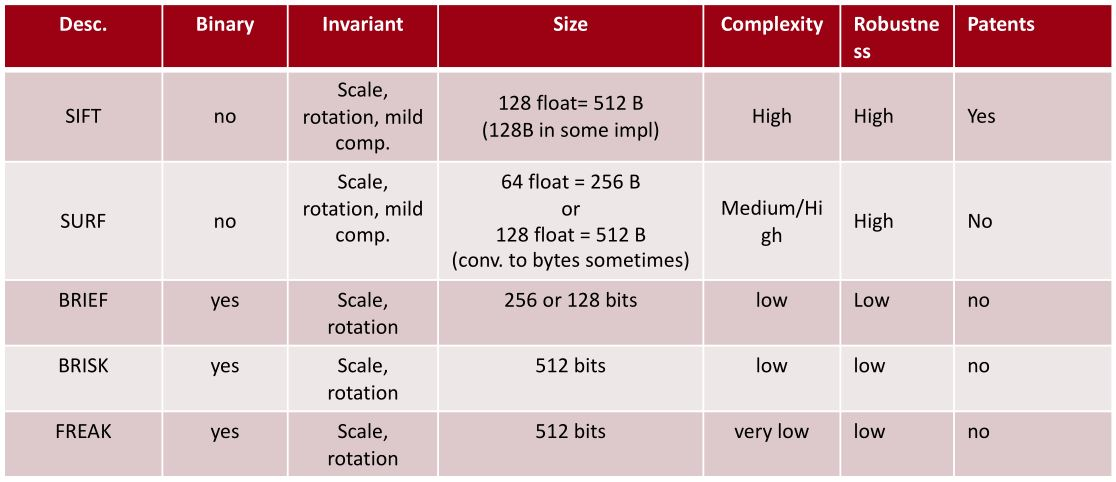
\includegraphics[width=0.9\textwidth]{images/Descriptors.jpg}
    \caption{Common algorithms for feature description.}
    \label{fig:descriptors}    
\end{figure}

\subsection{What is an autoencoder}

What were our choices (programming language,...) cons of using matlab as a Machine Learning tool
The objective of the project is